\documentclass[
    letterpaper,
    12pt,
    openbib,
]{memoir}

\usepackage{tabularx}
\usepackage{palatino}
\usepackage{blindtext}
\usepackage{xspace}
\usepackage{siunitx}
\usepackage{mhchem}
\usepackage{braket}
\usepackage{cite}
\usepackage{nicefrac}
\usepackage{bm}
\usepackage{glossaries-extra}
\usepackage{cleveref}

\bibliographystyle{ieeetr}

% Lengths
\newlength{\linespace} \setlength{\linespace}{\baselineskip}
\newlength{\topfiddle} \setlength{\topfiddle}{2\linespace}


\newcommand{\defendmonth}{May\xspace}
\newcommand{\defendday}{?\xspace}
\newcommand{\defendyear}{2024\xspace}
\newcommand{\defenddate}{\defendmonth \defendday, \defendyear}

\newcommand{\pretoctitle}[1]{{\Large\bfseries\clearpage\vspace{\topfiddle}#1\par\vspace{\topfiddle}}}
\newcommand{\acknowledgements}{\pretoctitle{Acknowledgements}}
\newcommand{\preface}{\pretoctitle{Preface}}

\newcommand{\etal}{\textit{et al.}\xspace}

\newcommand{\onlinecref}[1]{Ref.~\citenum{#1}\xspace}


\newabbreviation{afm}{AFM}{antiferromagnetic}
\newabbreviation{cdw}{CDW}{charge density wave}
\newabbreviation{shg}{SHG}{second harmonic generation}
\newabbreviation{trshg}{tr-SHG}{time resolved second harmonic generation}

\newcommand{\suchthat}{\mathrm{s.t.}}
\newcommand{\tastwo}{$1$\textit{T}-\ce{TaS2}}

\newtheorem{theorem}{Theorem}[section]


\chapterstyle{brotherton}


\begin{document}

\frontmatter*
\begin{titlingpage}
\calccentering{\unitlength}
\begin{adjustwidth*}{\unitlength}{-\unitlength}
\centering
{\Large\bfseries Ultrafast spectroscopy and control of correlated quantum materials}\\[0.5\baselineskip]
{By}\\[0.5\baselineskip]
{\large Bryan T. Fichera\\[0.5\baselineskip]}
{B.S., University of Pennsylvania (2017)\\[0.5\baselineskip]
Submitted to the Department of Physics\\ in partial fulfillment of the requirements for the degree of\\[0.5\baselineskip]
{\large Doctor of Philosophy\\[0.5\baselineskip]}
at the\\[0.5\baselineskip]
{\large MASSACHUSETTS INSTUTITE OF TECHNOLOGY\\[0.5\baselineskip]}
\defendmonth\defendyear\\[0.5\baselineskip]}
\copyright Bryan Thomas Fichera, \defendyear. All rights reserved.\\[0.5\baselineskip]
The author hereby grants to MIT a nonexclusive, worldwide, irrevocable, royalty-free license to exercise any and all rights under copyright, including to reproduce, preserve, distribute and publicly display copies of the thesis, or release the thesis under an open-access license.\\[2\baselineskip]
\flushleft
\begin{tabularx}{\textwidth}{ll}
Authored by: & Bryan T. Fichera\\
& Department of Physics\\
& \defenddate\\
\\
Certified by: & Nuh Gedik\\
& Donner Professor of Physics, Thesis supervisor\\
\\
Accepted by: & ?\\
& ? Professor of ?\\
& ? Chair of ?
\end{tabularx}
\end{adjustwidth*}
\end{titlingpage}

\begin{abstract}
\blindtext
\end{abstract}

\acknowledgements
\blindtext

\clearpage
\preface
The physics of solids is, to me, one of the most important and fundamental fields of modern science.
This might seem, to some, a bit of a hot take.
After all, by studying condensed matter physics, one learns next to nothing about, say, the formation of the stars and planets, or the origin of the universe.
Nor does one learn about life, death, consciousness, disease, ethics, God, or any other question that perhaps puzzled humanity prior to about five hundred years ago.
Certainly no one would argue that condensed matter physics is quite \emph{useless}, given that nearly every device we interact with in modern life required some condensed matter physicist somewhere along the way to make one brilliant discovery or another---yet when the human mind starts to wander, and our thoughts turn to the metaphysical, we tend to look up, not down.

In my work I have taken a quite different view.
Condensed matter physics, to me, is ultimately the study of how \textit{truly boring} objects, when brought together in large quantites, \textit{become} interesting, seemingly in spite of themselves.
When electrons are put together in a lattice and allowed to interact slightly with the massive nuclei, at low enough temperatures they pair, the low-energy excitations become gapped, and current can flow for infinite times and with absolutely zero energy loss.
Those same electrons, with some other set of interactions, may instead ionize (the opposite of pairing!) to create an electrically insulating state, whose low-energy excitation spectrum is nevertheless gapless and consisting of charge-neutral spin-$\nicefrac{1}{2}$ particles.
In all such cases, these systems exist in otherwise ordinary-looking rocks, fit in the palm of a hand\footnote{Hopefully, gloved.}, and are more or less indistinguishable from something you might find sticking into the bottom of your shoe.

While such systems may not tell us a lot\footnote{
    This discussion is obviously intentionally reductive.
    In truth there is still quite a bit one can learn about, e.g. the early universe by studying condensed matter physics, see the \citet{kibble_introduction_2008}.
}
about the early universe, considering these and related problems lets us ask deep, fundamental questions about the world we live in---like, why is this thing a metal, but this thing is an insulator? What do those terms even mean?---that I don't think we would try to ask otherwise.
To me, focusing our attention on these problems, despite their obviously terrestrial nature, is not a waste of time; rather, I think they remind us that even the most mundane aspects of the human experience involve a level of complexity far beyond what we are capable of understanding absent the pursuit of science.

Throughout the seven years of my Ph.D., I hope to have made a few contributions to this pursuit.
As the title of this work implies, I have mainly focused on the application of ultrafast techniques to the study of correlated quantum materials, which I loosely define as those materials in which the interaction between particles is large enough so as to compete with the kinetic energy of those particles.
It is in these materials that I think lies the true frontier of condensed matter physics; here, much of our basic intuition about non- or weakly-interacting theory fails, and more complicated notions of phase competition, phase separation, disorder, pairing, coherence, etc. are needed to property describe the relevant physics.

In my own view, and in the view of many scientists in this field\citep{alexandradinata_future_2022}, the main question for strongly correlated physics amounts to: ``Given a correlated system with some defined combination of different interaction strengths, is there a general theory which allows us to predict the phase diagram of this system \textit{a priori}?''
Related of course are questions about the origins of high-$T_c$ superconductivity, strange metallicity, quantum spin liquids, and other exotic phases that we find emerging from strongly interacting systems.
Since such a theory does not currently exist, at least with the level of predictive power that I think most would find satisfactory, new advances in this field typically come directly from experiment.
Ultrafast optics plays a special role in this regard, for reasons that I will explain in \cref{ch:intro}.

Progress thus happens in this field somewhat unsystematically, with small pieces of the puzzle added at random, but not infrequenct, intervals.
Usually it is either new techniques or new materials that are the driving force here.
To this end, I have tried to pursue both directions in my Ph.D.
Appearing also in \cref{ch:intro} is thus a description of the materials I studied the most during my thesis, two of them, \ce{CuBr2} and \ce{CaMn2Bi2} I consider criminally understudied.
On the technique side, almost all of the work presented in this thesis was done using \gls{trshg}, a relatively new, nonlinear optical technique which, at the most basic level, probes the point group assumed by the charge distribution function $\rho(\bm{x})$ at any given point in time.
\Gls{shg} and \gls{trshg} are tricky techniques, with many pitfalls both practically and theoretically; \cref{ch:shgtheory,ch:shgpractice} are thus devoted to what I hope is a useful, if not fully compehensive, description of the technique.
\Cref{ch:polrotators} is devoted to work that we did developing a new way to control the polarization of the light in a \gls{trshg} experiment using stepper motors.
My hope is that these chapters are useful not only for the new student trying to build their own setup or analyze their own \gls{shg} data, but also for people for whom \gls{shg} is not a focus but nevertheless want to learn about it in slightly more detail than one would get from a typical paper or review article.

What follows, then, is a description of the three main research works I contributed during my Ph.D..
The first, which I describe in \cref{ch:tastwo}, involves work that I did during my second and third years on \tastwo, a very interesting \gls{cdw} material that, among other things, undergoes a mirror symmetry breaking \gls{cdw} transition at $350$ \si{K} that shows up in the \gls{shg} as a sudden distortion of the flower pattern at that temperature.
Since this transition breaks mirror symmetry, two energetically degenerate domains should be present, corresponding to two opposite planar chiralities; in this work, we showed that \gls{shg} could differentiate between these two domains (i.e. the flower pattern in either domain looks different).

The second and third works, which I describe in \cref{ch:cmb,ch:cubr2}, in contrast to the \tastwo work, both involve taking the system out of equilibrium to study the dynamics.
In \ce{CaMn2Bi2} (\cref{ch:cmb}), we discovered that photoexcitation causes the \gls{afm} order in that compound to reorient (relative to equilibrium) to a metastable state which is impossible to reach from the equilibrium state thermodynamically.
Light is thus used to \textit{control} the magnetic order in this material.

In \ce{CuBr2} (\cref{ch:cubr2}), light is not used to control the order parameter like in \ce{CaMn2Bi2}, but it does excite coherent oscillations of the collective modes of the multiferroic order (electromagnons), whose frequency, amplitude, damping, etc. may be probed in \gls{trshg} as a function of temperature---a methodology referred to as ultrafast \textit{spectroscopy}.
In doing so, we found that one of these collective modes is actually quite special, as it is in fact the analogue of the Higgs mode of particle physics in the context of a multiferroic material.

I conclude with various remarks in \cref{ch:conclusion}, as well as an appendix, in which I enumerate briefly all of the null-result experiments I performed during my Ph.D., in the hopes that future scientists don't have to waste time on what we already know are fruitless pursuits.
If you have any questions about this or any other section of this thesis, please do not hesitate to reach out via email.

\clearpage

\tableofcontents
\clearpage
\listoffigures
\clearpage
\listoftables
\clearpage

\mainmatter*
\chapter{Ultrafast optics in correlated electron systems\label{ch:ch1}}
\blindtext

\chapter{Second harmonic generation: theory\label{ch:ch2}}
\blindtext

\chapter{Second harmonic generation: practical}
In the last chapter we saw that the \gls{shg} intensity in a given crystal is related to the point group, order parameter, band structure, etc. of that crystal via the susceptibility tensor $\chi_{ijk}$.
It is also obvious from \cref{sec:neumann} that the ideal scenario is to be able to measure as many of the numbers $\chi_{ijk}$ as possible; after all, if you only measured the $xx$ component of \cref{eq:c2eps,eq:d3deps}, you would have obtained essentially no information about your crystal whatsoever.
The \gls{shg} setup that we built (whose design is mostly credited to Torchinsky and Hsieh\citep{torchinsky_low_2014}, with some improvements by us which I will discuss below) was designed with exactly this goal in mind.
There are two key insights which make this design work: one, the light is obliquely incident on the sample so there is some component of $\bm{E}^\mathrm{in}$ directed along the sample normal, and two, we rotate the plane of incidence so that the in-plane field direction sweeps an entire $360^\circ$.
The first point allows us to measure elements of $\chi_{ijk}$ with $z$ indices\footnote{Here and unless otherwise noted I define the sample normal to be the $z$ axis.}, and the second point makes sure we get all of the $x$ and $y$ elements of $\chi_{ijk}$ too.
All of the tensor elements are thus given a chance to contribute to the \gls{shg} intensity in a given experiment.

With those considerations in mind, let me proceed to give a schematic description of our \gls{shg} setup.
Some of the choices we made may seem arbitrary right now, but I will go over them in detail in \cref{sec:beforeyoubuild}.
The starting point is our regenerative amplifier (Spectra-Physics Spitfire Sptf-100f-5k-xp), which produces $100$ \si{fs} $800$ \si{nm} pulses at a $5$ \si{kHz} repetition rate from an $86$ \si{MHz} seed laser (Spectra-Physics Tsunami 3941-M1S). 
$90\%$ of the beam is split off to power an \gls{opa}, and the remaining $10\%$ is used for the \gls{shg} probe beam.
After passing through an optical telescope, which creates a collimated beam of width $1-2$ \si{mm}, this beam is attenuated with a polarizer - half-wave plate - polarizer triplet, and then elliptically polarized with a quarter-wave plate and half-wave plate in series.
The ellipticity at this stage is set so the light is perfectly circularly polarized following transmission through a phase mask, as described below.

After passing through these polarization optics, the beam is focused with a lens onto the aforementioned phase mask, which acts as a transmissive diffraction grating and separates the beam into multiple different diffraction orders.
The $+1$ order diffraction comes off at an angle of roughly $7^\circ$, while the other orders are blocked with anodized aluminum foil. 
This (diverging) beam then propogates at $7^\circ$ to the optical axis before meeting a lens set at the appropriate distance so as to both collimate the beam and rectify the $7^\circ$ progation angle.
Then, the light passes through a dichroic mirror (which transmits $800$ \si{nm} and reflects $400$ \si{nm}), becomes linearly polarized by a wire-grid polarizer, and is then focused onto the sample at a $10^\circ$ angle of incidence by passing through the edge of a $1$ \si{in}-diameter $50$ \si{mm} achromatic focusing lens.
The interaction between the light and the sample causes \gls{shg} to be radiated in reflection at the same $10^\circ$ angle of incidence, so that the \gls{shg} beam passes through the opposite side of the $50$ \si{mm} lens before passing through a second, independent polarizer which is used to control the polarization of the measured light.

\begin{figure}
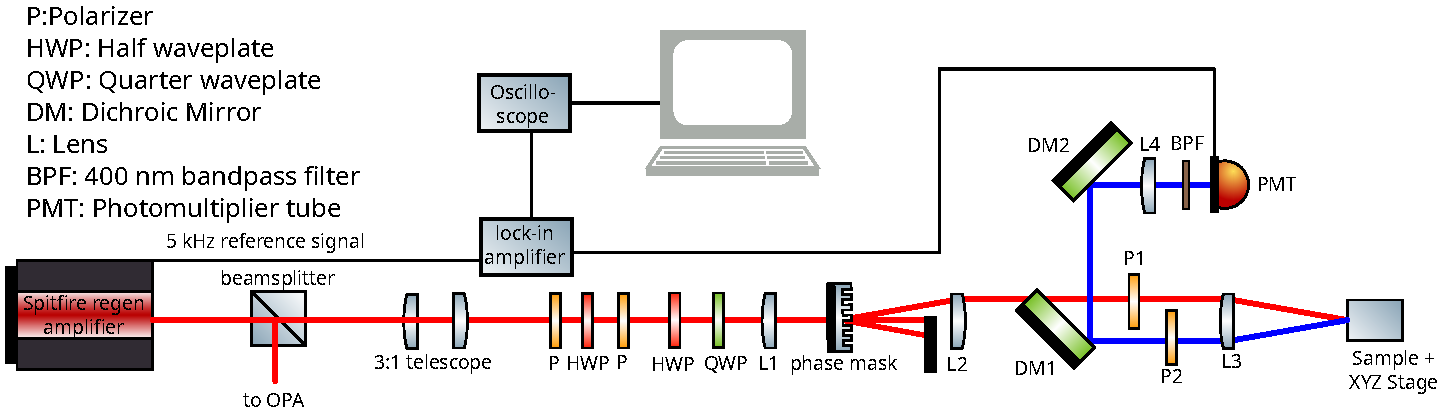
\includegraphics[width=\textwidth]{gfx/ch3/pdf/setup.pdf}
\caption{\label{fig:setup}Schematic drawing of the \gls{shg} setup used in this research. After \citet{morey_automated_2024}.}
\end{figure}

Finally, the polarized output reflects off of two dichroic mirrors (oriented in such a way as to cancel the differing effect of the Fresnel equations on the reflectivity of S and P polarized light) and is focused through a $400$ \si{nm} bandpass filter onto a \gls{pmt} by a $400$ \si{mm} lens.
The current output of the \gls{pmt} is filtered by a lock-in amplifier (for static \gls{shg}, set to the $5$ \si{kHz} repetition rate of the laser) and read out on an oscilloscope.
The phase mask, incoming polarizer, and outgoing polarizer are mounted on rotating lens tubes which are connected via pulley to a common motor shaft driven by a brushless DC motor.
The motor thus continuously rotates the plane of incidence of the experiment, since the latter is entirely defined by the phase mask and the polarizers.
The rotation angle is tracked as a function of time by an optical rotary encoder, consisting of a laser pointer passed through a chopper wheel (with 100 slots) mounted at the end of the motor shaft and detected via photodiode.
The encoder signal and the lock-in signal are both sent to a homemade oscilloscope (an Arduino Uno microcontroller which separates the lock-in signal into different individual rotations by looking for peaks in the encoder signal), the output of which is sent to a computer for further data processing.

\section{Before you build}\label{sec:beforeyoubuild}

I list here a few essential aspects of \gls{shg} that should be considered before designing a new setup.

\subsection{Spot size}

One of the most important quantities in an \gls{shg} setup is the diameter of the probe spot.
Ideally, this diameter is as small as possible, so as to measure the smallest samples or domain sizes.
However, there is an important caveat: for constant fluence (i.e. supposing we are limited by the sample damage threshold), the \gls{shg} signal to noise ratio scales linearly in the area excited by the probe, and thus \gls{shg} microscopes have a difficult time measuring small \gls{shg} signals compared to traditional \gls{shg} setups with a larger excitation area.
To see this, let us say that our detector measures the number of photons per \gls{shg} pulse, which is proportional to the pulse energy $U_p(2\omega)$.
Assuming the input and output pulse intensity profiles have the shape of a square wave with width $\tau$ and height $I_p(\omega)$ and $I_p(2\omega)$, respectively, we have
\begin{equation}
U_p(2\omega) = A I_p(2\omega) \tau
\end{equation}
and
\begin{equation}
U_p(\omega) = A I_p(\omega) \tau
\end{equation}
where $A$ is the area of the beam at the sample surface.
The \gls{shg} intensity is proportional to the square of the input intensity
\begin{equation}
I_p(2\omega) \propto I_p^2(\omega)
\end{equation}
so that
\begin{equation}
U_p(2\omega) \propto \frac{U_p^2(\omega)}{A\tau}.
\end{equation}
Substituting for the fluence $f$
\begin{equation}
f(\omega) = \frac{U_p(\omega)}{A}
\end{equation}
we have
\begin{equation}
U_p(2\omega) \propto \frac{f^2(\omega)A}{\tau}
\end{equation}
i.e., if we hold the fluence constant at the sample damage threshold, the number of photons in the generated \gls{shg} pulse is proportional to the excitation area and inverse to the pulse width.
The signal to noise ratio is then given by
\begin{equation}
\mathrm{SNR} \propto \frac{U_p(2\omega)}{\sqrt{r}}
\end{equation}
where $r$ is the system repetition rate.

\subsection{Oblique vs. normal incidence}

While all of the results presented in this thesis utilized the setup in \cref{fig:setup}, where the incident beam makes a small angle with respect to the sample normal, plenty of groups use a different approach where that angle is set to $0^\circ$.
This has the obvious disadvantage of not specifying all of the tensor elements, since any element $\chi_{ijk}$ with $i, j, k = z$ is not accessible in this geometry.
However, in some cases this can actually be something of an advantage.
For example, sometimes unwanted \gls{shg} contributions (see \cref{sec:manyshgterms}) may be avoided in the normal incidence geometry, assuming the \gls{na} of the focusing optic is small enough that longitudinal components of the electric field are nearly zero.
Furthermore, in some materials the order parameter only couples to one or two elements of $\chi_{ijk}$; if none of these elements have a $z$ index, it is needless to complicate the analysis with oblique incidence.

In my experience, oblique incidence seems to be useful in two broad cases.
For one thing, some order parameters only show up in the $z$ components of $\chi_{ijk}$ (this is the case in \tastwo, see \cref{sec:tastwo}), in which case one obviously needs a nonzero angle of incidence to access these components.
A more subtle point is that, even if in practice all of the phenomenology of a particular sample only shows up in the $x$ and $y$ indices of $\chi_{ijk}$, still one must measure the full tensor to \emph{rule out} unseen phenomenology in the other indices.
Both the \ce{CaMn2Bi2} (\cref{ch:ch5}) and \ce{CuBr2} (\cref{ch:ch6}) works presented in this thesis are examples of exactly this point, where the main scientific arguments involve either comparing \gls{shg} patterns in two domains or comparing oscillation amplitudes in different polarization channels.
Clearly one needs to know all of the tensor elements to make those arguments exact.

\chapter{Second harmonic generation as a probe of broken mirror symmetry in 1\textit{T}-\ce{TaS2}}
\chapter{Light-induced reorientation transition in the antiferromagnetic semiconductor \ce{CaMn2Bi2}}
\chapter{Amplitude-mode electromagnon in the XXZ chain \ce{CuBr2}}
\chapter{Concluding remarks}

\backmatter*
\begin{thebibliography}
\bibliography{bibliography.bib}
\end{thebibliography}

\end{document}
